% You should title the file with a .tex extension (hw1.tex, for example)
\documentclass[a4paper, 11pt]{article}

\usepackage{amsmath}
\usepackage{amssymb}
\usepackage{fancyhdr}
\usepackage{graphicx}
\usepackage{scribe}
\usepackage{graphicx}
\usepackage[margin=1in]{geometry}
\usepackage{graphicx}
\newcommand{\question}[2] {\vspace{.25in} \hrule\vspace{0.5em}
\noindent{\bf #1: #2} \vspace{0.5em}
\hrule \vspace{.10in}}
\renewcommand{\part}[1] {\vspace{.10in} {\bf (#1)}}

\newcommand{\myname}{Kriangsak Thuiprakhon}
\newcommand{\myemail}{kriangsak.thi@student.mahidol.edu}
\newcommand{\myhwnum}{}

\setlength{\parindent}{0pt}
\setlength{\parskip}{5pt plus 1pt}
 


\begin{document}

\medskip                        % Skip a "medium" amount of space
                                % (latex determines what medium is)
                                % Also try: \bigskip, \littleskip

\thispagestyle{plain}
\begin{center}                  % Center the following lines
{\Large ICCS481: Midterm Exam } \\
\myname \\
\myemail \\
\end{center}

\question{1}{UNSTARING}
In order for any sequences of  N operation ( \textsc{addvertex}, \textsc{addEdge},\textsc{unstar}) to deliver in linear time, it means that we need to show that it takes amortized constant time per operation.
\begin{lemma}
Any sequence of sequences of N operation ( \textsc{addvertex}, \textsc{addEdge},\textsc{unstar}) take O(n) 
\end{lemma}
\begin{proof}
We will prove this lemma using the potential method. First, let us define the potential function:
$$\phi^{(i)} = \sum_{u} [deg(u)-3] \text{ For all u where deg(u)} \geq 3$$

It is obvious to see that the above function will always be positive 
Now we will use this function to show that the amortized cost per one of the above iterations takes constant time.
recall the equation of the amortized cost( $\hat{c}$) where c denotes the actual cost per iteration.
$$\hat{c} = c + \Delta \phi$$
\begin{itemize}
\item For \textsc{addvertex} 
 \begin{align*}
 \hat{c} & = c + \Delta \phi\\
 &= 1 + \phi^{(i)} -\phi^{(i-1)} \\
 &= 1 + \phi^{(i)} -\phi^{(i)} \\
 &=1\\
 & =O(1)
 \end{align*}
\item For \textsc{addEdge}. There are two cases to consider:
	\begin{itemize}
	\item the case when adding an edge but every node in graph \textsc{G} still has degree less than 3. In this case, it is the same as what is being done in \textsc{Addvertex} Operation since there is no change in the potential function:( i.e., the potential function does not change because there is no node that will have a degree greater than 3).
	\item The case when adding an edge and it turns that node to be a node of degree greater than 3, (i.e., 4). then,  
	 \begin{align*}
 \hat{c} & = c + \Delta \phi\\
 &= 1 + \phi^{(i)} -\phi^{(i-1)} \\
 &= 1 + \phi^{(i)} -(\phi^{(i)} -1)\\
 &=2
 \\
 & =O(1)
 \end{align*}
	\end{itemize}
	\item For \textsc{unstar}) with a node of degree d.
	 \begin{align*}
 \hat{c} & = c + \Delta \phi\\
 &= d + \phi^{(i)} -\phi^{(i-1)} \\
 &= d + d(3-3) -(d-3) \\
 &=3\\
 & =O(1)
 \end{align*}
\end{itemize}
Since every function takes amortized constant time, we conclude that the sequence of N operation takes amortized O(N).
\end{proof} 

\question{2}{Parallel Sublinear-Work Approximate Median}
\part{i}
\begin{itemize}
\item Show that work bound is O(n)\\
\begin{proof}
From Data Structure, we did in the end analyze the running time of some flavor of $\varepsilon$-approximate median. We have proved the work bound:

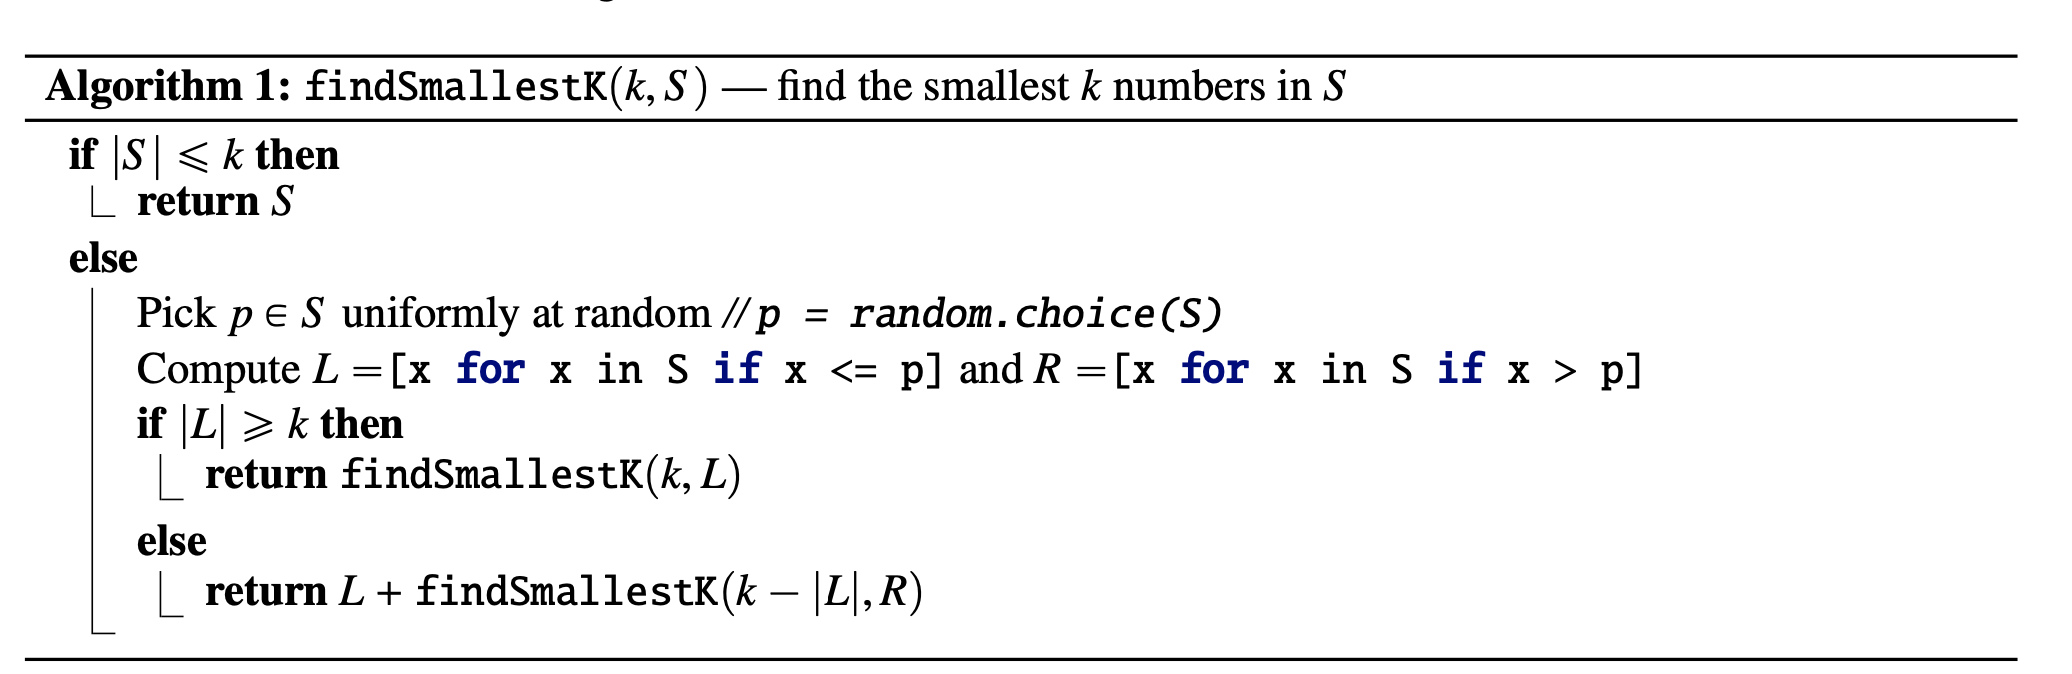
\includegraphics[width=\textwidth]{kmean.png}
Note that he picture is taken from DS lecture note by the same professor teaching this very class.
As we can see that the running time for this algorithm depends on  the size of the two arrays, L and R.
Let's write the recurrence  of work as:
$$W(n) = W(max(|L|,|R|)) + O(n) $$
From this on, we can see that our running time will be probabilistic, that is, we need to find the probability that the  length of them will fall in a good range, between $n/4$ to $3n/4$,which amounts to the $Pr[X_n  \leq \frac{3n}{4}]$ of $\frac{1}{2}$, denote $X_n = max(|L|,|R|)$. Now, if we denote the expected work  of the algorithm to be $\bar{W}$, then:
\begin{align*}
\bar{W} &\leq \mathbb{P}[X_n = i] \cdot \bar{W(i)} + cn \\
&\leq \mathbb{P}[X_n \leq 3n/4] \cdot \bar{W(3n/4)}  +\mathbb{P}[X_n > 3n/4] \cdot \bar{W(i)} + cn \\
\Rightarrow \bar{W} &\leq  \bar{W(3n/4)} +2 cn\\
\textmd{Which solves to O(n)}
\end{align*}
\end{proof}
\item Show that span bound is O($log^2n$)
\begin{proof}
In class, we can use \textsc{filter} to do the partition in L and R. and we proved that \textsc{filter} has span of O(logn). In the above algorithm, we can see that we can also see observe that we can partition up to at most $logn$ w.h.p. therefore, we have the span of this algorithm to be $O(log^2n)$
\end{proof}

\end{itemize} 
\part{ii} we can do so by doing pfor and since randomly picking a number and accessing an array take O(1), then we have work of O(T) and span of O(1)

\part{iii} We want to promise that what the algorithm returns has the rank between the given range.  That is:
$$Pr[ Y_i \in_R X \quad | \quad n(1/2+\varepsilon) \leq Rank_X(Y_i) \leq n(1/2+\varepsilon)] = 1 - 2\cdot Pr[Rank_X(Y_i) < n(1/2+\varepsilon)] -(*)$$
Using Union Bounds and symmetry,
Let Y denote an indicator random variable 
$$
Y_i = \begin{cases}
1 & \text{ if  } Rank_X(Y_i) < n(1/2 -\varepsilon) \\
0 &\textmd{ otherwise}
\end{cases}
$$
From this, what is the expectation of $Y$ ? To find the expectation of Y, we first need the find the probability that an element drown is bad, by bad i mean, is not in the range of approximate median. This is simply:
$$Pr[Rank_X(Y_i) < n(1/2 -\varepsilon)] = \frac{n(1/2-\varepsilon)}{n} = \frac{1}{2}-\varepsilon $$
By definition of expectation,
$$ \mathbb{E}[Y] = T(\frac{1}{2} -\varepsilon) $$

From now we can apply Chernoff-Hoffding bounds. We want something like $Pr[Y < T/2] $ and the expectation is  $\mu = T(\frac{1}{2} -\varepsilon) $. We need to massage it a little bit.
\begin{align*}
Pr[Y < \mu  + T\varepsilon] & \leq  exp\{-2\varepsilon^2 T\}\\
\end{align*}
This means in $*$ we have that 
$$Pr[ Y_i \in_R X \quad | \quad n(1/2+\varepsilon) \leq Rank_X(Y_i) \leq n(1/2+\varepsilon)] \leq 1 - 2exp\{-2\varepsilon^2 T\}$$
now we set:
$$\delta  = 2\cdot e^{-2\varepsilon^2 T} $$
Therefore, 
$$T = \frac{ln(\delta/2)}{-2\varepsilon^2}$$
\question{3}{JL}
\begin{enumerate}

\item For $0<t<1/2 $ if 	$R \in_R {-1,1}$ ,then  $\mathbb{E}[e^{tR}] \leq e^{t^2/2}$
\begin{proof}
By Definition of expectation,
\begin{align*}
\mathbb{E}[e^{tR}] &= \frac{1}{2}( e^{t} + e^{-t})\\
& =  \frac{1}{2}( \sum_{\text{k: even}}\frac{t^k}{k!}) \leq  \sum_{ k \geq 0}\frac{(t^2/2)^k}{k!} = e^{t^2/2}
\end{align*}
\end{proof}
\item show that $\mathbb{E} [e^{tV_i}] \leq e^{  \frac{1}{2} t^2 \cdot ||x||_2^2  } $
\begin{proof}
\begin{align*}
\mathbb{E} [e^{tV_i}] &= \mathbb{E} [e^{t\sum_{j=1}^D R_j xj}]\\
& = \Pi_{j=1}^D [\mathbb{E} [e^{(tx_j)R_j}]]\\
\text{from 1}\\
& \leq \Pi_{j=1}^D [e^{x^2t^2/2}]]\\
&\leq e^{ \frac{t^2 ||x||_2^2}{2}}
\end{align*}
\end{proof}
\item Let G ~ N(0,1). Show that 
$$
\mathbb{E}[e^{tG}] = e^{t^2/2}
$$
\begin{proof}
By definition of expectation of continuous  random variable:
$$
\mathbb{E}[e^{tG}] = \int_{-\inf }^{\inf} e^{tG} \cdot \frac{e^{-G^2/2}}{\sqrt{2\pi}} dG = e^{t^2/2}
$$
By Wolfram Alpha
\end{proof}
\item For $||x||_2^2 =1$, show that
$$
\mathbb{E} [e^{tV_i^2}] \leq \frac{1}{\sqrt{1-2t}}
$$
\begin{proof}
from the given convolution trick we have: 
\begin{align*}
\mathbb{E} [e^{tV_i^2}]  &= \mathbb{E}_G[ \mathbb{E}_V [e^{\sqrt{2t}GV}]]\\
& = \mathbb{E}_G[ e^{tG^2}] \textmd{ from 2}\\
&\leq \frac{1}{\sqrt{1-2t}} \textmd{ from the bound in class}
\end{align*}
\end{proof}
\end{enumerate}
\end{document}
